% Preamble ----------------------------------------

\documentclass{beamer}

\mode<presentation> {

  \usetheme{Singapore}

  %\setbeamertemplate{footline} % To remove the footer
  %\setbeamertemplate{footline}[page number] % To replace the footer
  \setbeamertemplate{navigation symbols}{} % To remove the navigation symbols
}
\AtBeginSection{\frame{\sectionpage}}

% Nag about bad practices.
\usepackage[l2tabu,orthodox]{nag}

% ----- Type & Spacing (==
% Set English hyphenation rules.
\usepackage{polyglossia}
\setdefaultlanguage{english}

% Font selection for XeTex and LuaLatex.
\usepackage{fontspec}
\defaultfontfeatures{Ligatures=TeX}

% Adjust micro-typography.
\usepackage{microtype}
\frenchspacing
%\hyphenpenalty=250

% Place all subscripts at the same height.
\usepackage{subdepth}
% ==)

% ----- Figures (==
\usepackage{graphicx}
\usepackage{booktabs}
% ==)

\definecolor{lgray}{gray}{0.6}


\title{2017 Data Mining Cup}
\author[2017 Team]{
  Lingfei Cui, \textcolor{lgray}{Weixiao Huang}, Shuhao Jiao,\\
  Haoran Li,   \textcolor{lgray}{Weitong Lin},   \textcolor{lgray}{Hugo Mailhot},\\
  Nick Ulle,   \textcolor{lgray}{Jiaping Zhang}, Jingyi Zheng
}
\institute[UC Davis]{University of California, Davis}
\date{\today}


% Slides ----------------------------------------
\begin{document}

\begin{frame}
  \titlepage
\end{frame}

\begin{frame}
  \frametitle{Overview} % Table of contents slide, comment this block out to remove it
  \tableofcontents
\end{frame}


\section{Introduction} % ----------------------------------------

\begin{frame}{2017 Data Mining Cup}
    \begin{itemize}
      \item Task released April 5th
      \item Use historical data to predict revenue for an online pharmacy
      \item Train on 90 days of user actions
      \item Predict revenue for each user action over subsequent 30 days
      \item Model with smallest squared error $\sum_i (r_i - \hat{r}_i)^2$ wins
    \end{itemize}
  We submitted predictions at 5:00am on May 17th!
\end{frame}

\begin{frame}{What do the data look like?}
  \begin{block}{Training Data -- train.csv} 
    \begin{itemize}
      \item Each of 2,756,003 rows is one user action for one product
        \begin{itemize}
          \item click, basket, or order
        \end{itemize}
      \item \texttt{revenue}, a multiple of \texttt{price}
      \item Other features:
        \begin{itemize}
          \item day, adFlag, availability, price, competitorPrice
        \end{itemize}
      \item No feature to identify distinct users
    \end{itemize}
  \end{block}

  \begin{block}{Test Data -- class.csv} 
    \begin{itemize}
      \item Same structure as above, excluding user action and \texttt{revenue}
      \item 1,210,767 rows
    \end{itemize}
  \end{block}
\end{frame}

\begin{frame}
  \frametitle{What do the data look like?}
  \begin{block}{Items Data -- items.csv} 
    \begin{itemize}
      \item Each of 22,035 rows is one item
      \item Information that doesn't change over time
      \item Linked to other data sets by product ID
      \item Other features:
        \begin{itemize}
          \item manufacturer
          \item group (``product group'')
          \item content, unit
          \item pharmForm, genericProduct
          \item salesIndex (``dispensing regulation code'')
          \item category, campaignIndex
          \item rrp
        \end{itemize}
    \end{itemize}
  \end{block}
\end{frame}

\section{Features \& Workflow} % ----------------------------------------

\begin{frame}{Feature Engineering}
  \begin{itemize}
    \item 113 new features (\sim 3000 after one-hot encoding)
    \item Based on intuition about and exploration of the data set
    \item Features that use labels generated separately to prevent leakage
    \item Discretized for CRF model
  \end{itemize}
\end{frame}

\begin{frame}{Important Features}
  \begin{itemize}
    \item Probability \texttt{order == 1} given current and previous
      \texttt{pid}
    \item Random effect encoding of day of week with nested \texttt{pid} 
    \item Likelihood encoding (odds ratio) of \texttt{pid}
    \item Probability of \texttt{pid} being ordered again
  \end{itemize}
\end{frame}

\begin{frame}{Workflow}
  We wrote about 35 scripts, excluding data exploration.
  \begin{block}{Scripts to:}
    \begin{itemize}
      \item merge data sets
      \item generate features
      \item fit models
      \item merge predictions
    \end{itemize}
  \end{block}
  We had scripts for cross-validation but ended up not using them.
\end{frame}

\begin{frame}{Workflow Flowchart}
  \begin{figure}
	  \centering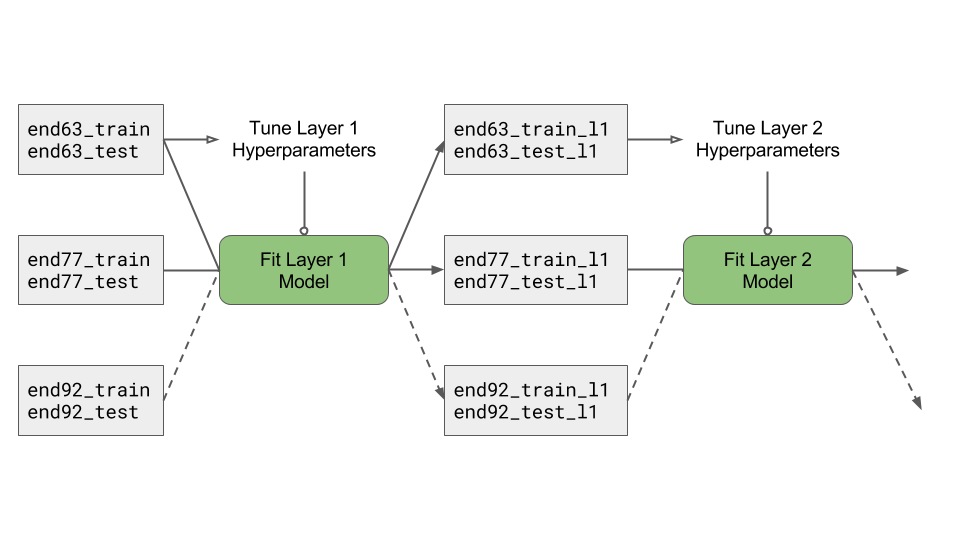
\includegraphics[scale=0.32]{graphics/data_flow_1.png}
  \end{figure}
\end{frame}

\begin{frame}{Workflow Flowchart}
  \begin{figure}
	  \centering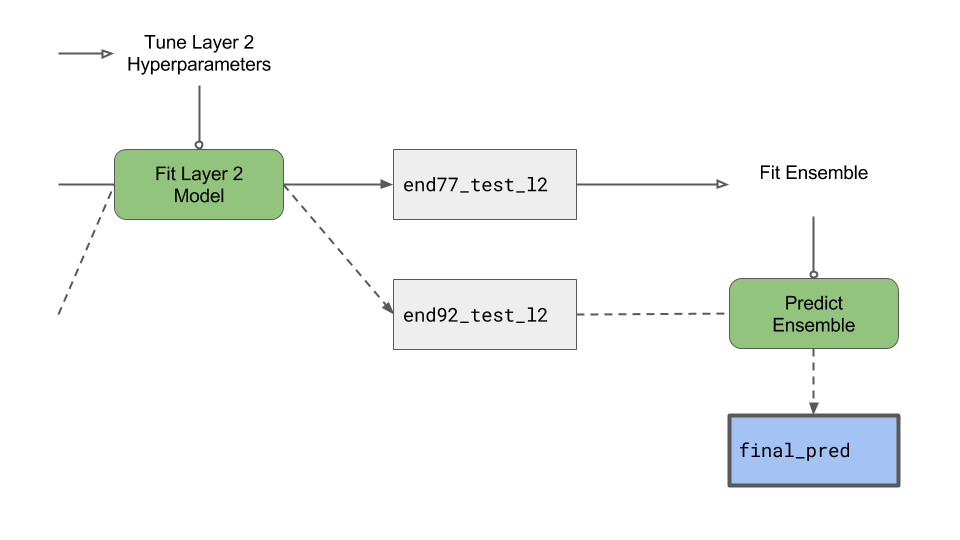
\includegraphics[scale=0.32]{graphics/data_flow_2.png}
  \end{figure}
\end{frame}

\section{Models} % ----------------------------------------

\begin{frame}{1st Layer}
  Predict \texttt{order}, which is binary.
  \begin{block}{Models}
    \begin{itemize}
      \item Conditional Random Field
      \item Generalized Linear Model
      \item \textcolor{lgray}{Gradient-boosted Machine}
      \item Neural Network
      \item Random Forests
      \item XGBoost
    \end{itemize}
  \end{block}
\end{frame}

\begin{frame}{2nd Layer}
  Predict \texttt{revenue} with 1st layer predictions as additional features.
  \begin{block}{Models}
    \begin{itemize}
      \item \textcolor{lgray}{Generalized Linear Model (Tweedie distribution)}
      \item \textcolor{lgray}{Gradient-boosted Machine}
      \item \textcolor{lgray}{Neural Network}
      \item XGBoost
    \end{itemize}
  \end{block}
\end{frame}

\begin{frame}{3rd Layer}
  \begin{itemize}
    \item Linear model for \texttt{revenue} based on 2nd layer models
    \item Weights for top 2 XGBoost models
    \item No other features included
    \item Manually corrected \texttt{availability == 4} to 0 revenue
    \item Estimated RMSE: 9.898
  \end{itemize}
\end{frame}

\section{Conclusion} % ----------------------------------------

\begin{frame}{What We Learned}
  \begin{itemize}
    \item Get something done at every meeting
    \item Get error estimates quickly (fit models early)
    \item Generate features that expose dependence structure to models
    \item Improve features based on weaknesses of fitted models
    \item Know how long models will take to tune and fit
  \end{itemize}
\end{frame}

\end{document} 
